\subsection{Configuration Distribution Protocol}

The dCAMP configuration distribution algorithm adheres to the Clustered Hashmap Protocol
(\url{http://rfc.zeromq.org/spec:12/CHP}) with a few minor (and one major) modifications:

\begin{enumerate}
\item only the Root node may write new configuration changes,
\item the full configuration table will be replicated across all first-level Collector nodes (lower-level nodes may
      filter their configuration to only store relevant data),
\item a different set of command names are used (as described below), and
\item configuration updates are distributed via the dCAMP hierarchy (instead of directly from the Root node).
\end{enumerate}

A newly assigned first-level Collector node will first subscribe to new configuration updates from the Root node and
then send a configuration snapshot request to the Root node. A newly assigned Sensor (or non-first-level Collector) node
will first subscribe to new configuration updates from its parent Collector node, and then send its parent Collector
node a filtered configuration snapshot request. Once its snapshot has been successfully received, a node will process
any pending configuration updates and then, in the case of a Collector node, respond to child node snapshot requests.

\begin{figure}[b]
    \centering
    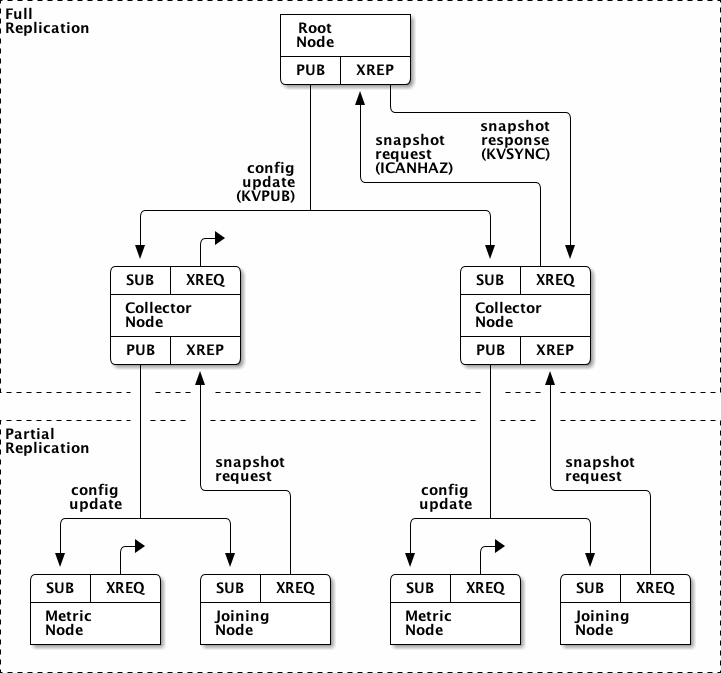
\includegraphics[scale=0.5]{config.png}
    \caption{Configuration Protocol Diagram}
    \label{fig:proto_config_image}
\end{figure}

\textit{In the following ABNF specification, \texttt{P-} represents the parent node (Root or Collector) sending a
message and \texttt{C-} represents the child node sending a message.}

\begin{figure}[h]
    \centering
    \begin{lstlisting}
    config-distribution = *update / snap-sync
    
    update              = P-KVPUB / P-HUGZ
    snap-sync           = C-ICANHAZ *P-KVSYNC ( P-KTHXBAI / P-WTF )
    \end{lstlisting}
    \caption{Configuration Protocol}
    \label{fig:proto_config_image}
\end{figure}

\subsubsection{Message Definitions}

These messages come from the CHP protocol. Additionally, a WTF error message may be sent by the parent in case of error.
It should be noted, each of the following messages is really the same five-frame format with varying key values and
semantics.

\textbf{ICANHAZ} \\
configuration snapshot request

\begin{lstlisting}
Frame 0: "ICANHAZ"
Frame 1: sequence number, 8 bytes in network order
Frame 2: <empty>
Frame 3: <empty>
Frame 4: subtree specification
\end{lstlisting}

\textbf{KVSYNC} \\
snapshot sync message

\begin{lstlisting}
Frame 0: key, as 0MQ string
Frame 1: sequence number, 8 bytes in network order
Frame 2: <empty>
Frame 3: <empty>
Frame 4: value, as blob
\end{lstlisting}

\textbf{KTHXBAI} \\
end of successful snapshot sync

\begin{lstlisting}
Frame 0: "KTHXBAI"
Frame 1: sequence number, 8 bytes in network order
Frame 2: <empty>
Frame 3: <empty>
Frame 4: subtree specification
\end{lstlisting}

\textbf{KVPUB} \\
configuration update sent from parent to child

\begin{lstlisting}
Frame 0: key, as 0MQ string
Frame 1: sequence number, 8 bytes in network order
Frame 2: UUID, 16 bytes in network order
Frame 3: properties, JSON-encoded, as 0MQ string
Frame 4: value, as blob

properties = ...
\end{lstlisting}

\textbf{HUGZ} \\
heartbeat message sent from parent to child (when no config updates)

\begin{lstlisting}
Frame 0: "HUGZ"
Frame 1: 00000000
Frame 2: <empty>
Frame 3: <empty>
Frame 4: <empty>
\end{lstlisting}
